\section{Implementation}
\label{sec:impl}

For implementation we have made use of the technique proposed by Ghassabani et al. \cite{Ghass16} for the efficient computation of IVCs, where there are two detailed algorithms for computing minimal IVCs: (1) Algorithm \ucbfalg that computes a MIVC of a given property, which is expensive. (2) Algorithm \ucalg that computes an \emph{approximately minimal} IVC in a much more efficient way.
%This section provides a high-level representation of these algorithms, and their implementation in a tool chain.
%
%\subsection{Algorithms}
%IVCs are built upon inductive proofs. In order to prove a property, inductive proof methods employ heuristics to derive additional lemmas (or invariants) so to strengthen the property and prove it inductively. To extract IVCs, the baseline algorithm \ucalg (Algorithm \ref{alg:uc}) iteratively uses UNSAT cores (hence the `UC') to determine an approximately minimal set of model elements.
%Algorithm \ref{alg:uc}
%first proves the property and obtains all the invariants generated for the proof (line 1). Since not all these invariants are essential for the proof, it performs a minimization step to keep a set of necessary invariants (line 2). The proofs of these invariants themselves are dependent on the structure of the model or design elements that we have defined them as Inductive Validity Core (Definition \ref{def:ivc}).
%So, using function $map\_to\_design$, Algorithm \ref{alg:uc}
%computes those design elements. Finally, the algorithm minimizes the computed elements to obtain an approximately minimal IVC (line 4).
%Although Algorithm \ref{alg:uc} performs minimization, because of the structure of the inductive proofs, \ucalg might still not produce a minimal IVC. It is often the case that to discover a minimal proof, additional lemmas might be necessary that were not part of the original proof.  It can also be the case that different minimal lemma sets may require larger or smaller sets of model elements.
%%Ela: we will add back this footnote after the review process
%% UPDATE: I add this back since I moved the other footnote
\footnote{For complete information, see Ghassabani et. al \cite{Ghass16}.}
%--------------------------
%Ela: I commented the above footnote because it gives everything away when being
%read right before the next footnote.
%Besides, we put ourselves into trouble. Again, they may try hard to find fault with us.
%And this gives them a hint why you didn't explain the algorithms in detail...
%-------------------------
%Therefore, Algorithm \ref{alg:ucbf}, \ucbfalg, includes a minimization brute-force post-processing step starting from the result of \ucalg (hence `UCBF').  The results from the \ucbfalg\ algorithm are guaranteed to be minimal.
Figure \ref{alg:must} is also an efficient way of computing the \emph{must} set of a given property using \ucalg. A different algorithm for computing $MUST (P)$ is to first compute $AIVC (P)$ and then take the intersection of all sets in $AIVC (P)$, which requires an algorithm for finding $AIVC$.  However, n{\"a}ive approaches for computing all inductive validity cores would be very inefficient.

Note that, as discussed in Section \ref{sec:method}, the
output of \ucalg (as well as \ucbfalg) for $(I, T) \vdash P$ pinpoints the covered design elements
using \ivccov\ (Definition \ref{def:coverage-justi}).
And, the output of \mustalg represents covered design elements according to \nondetcovalt\ (or \nondetcov ), which is the same as $MUST(P)$.
%
%\vspace{-0.1in}
%\begin{algorithm}
%  \SetKwInOut{Input}{input}
%  \SetKwInOut{Output}{output}
%  \Input{$(I, T) \vdash P$}
%  \Output{(Approximately) minimal IVC for $(I, T) \vdash P$}
%  \BlankLine
%  $Invs \leftarrow get\_inductive\_invariants((I, T), P)$ \\
%  $Invs \leftarrow minimize(Invs)$ \\
%  $S \leftarrow map\_to\_design (T, Invs)$ \\
%  $S \leftarrow minimize(S)$ \\
%  \Return{S}
%\caption{An abstract representation of \ucalg \cite{Ghass16}}
%\label{alg:uc}
%%\vspace{-0.1in}
%\end{algorithm}

%\begin{algorithm}
%  \SetKwInOut{Input}{input}
%  \SetKwInOut{Output}{output}
%  \Input{$(I, T) \vdash P$}
%  \Output{Minimal IVC for $(I, T) \vdash P$}
%  \BlankLine
%  $S \leftarrow \ucalg((I, T) \vdash P)$ \\
%  \For{$x \in S$} {
%    \If{$(I, S\setminus\{x\}) \vdash P$}{
%      $S \leftarrow S\setminus \{x\}$
%    }
%  }
%  \Return{S}
%\caption{An abstract representation of \ucbfalg \cite{Ghass16}}
%\label{alg:ucbf}
%\end{algorithm}

%\begin{algorithm}
%  \SetKwInOut{Input}{input}
%  \SetKwInOut{Output}{output}
%  \Input{$(I, T) \vdash P$}
%  \Output{Must set for $(I, T) \vdash P$}
%  \BlankLine
%  $S \leftarrow \ucalg((I, T) \vdash P)$ \\
%  $M \leftarrow \varnothing$ \\
%  \For{$x \in S$} {
%    \If{$(I, T\setminus\{x\}) \nvdash P$}{
%      $M = M \cup \{x\}$
%    }
%  }
%  \Return{M}
%\caption{\mustalg: an algorithm to compute $MUST(P)$ for a given $P$}
%\label{alg:must}
%\end{algorithm}
\begin{figure}
  \centering
  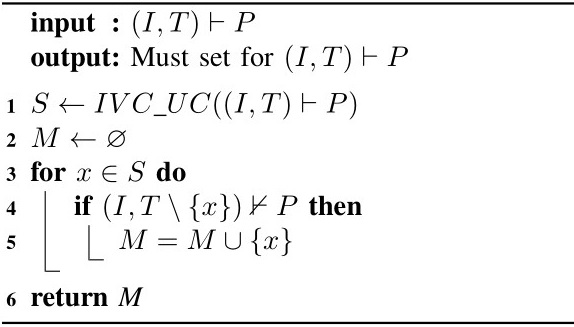
\includegraphics[width=0.7\columnwidth]{figs/mustalg.jpg}
  %\vspace{-0.2in}
  \caption{an algorithm to compute $MUST(P)$ for a given $P$}\label{alg:must}
\end{figure}
%
%\subsection{Tooling}
%
The three introduced algorithms have been implemented in the \texttt{JKind} model checker~\cite{jkind}, which is an infinite-state industrial model checker. \texttt{JKind} proves safety properties using multiple cooperative engines in parallel including $k$-induction \cite{SheeranSS00}, property directed reachability (PDR) \cite{Een2011:PDR}, and template-based lemma generation \cite{Kahsai2011}. It accepts
Lustre programs written over the theory of linear integer and real
arithmetic. In the back-end, it uses an SMT solver such as
Z3 \cite{DeMoura08:z3}, Yices \cite{Dutertre06:yices},
MathSAT \cite{Cimatti2013:MathSAT}, or SMTInterpol \cite{Christ2012:SMTInterpol}.
\texttt{JKind} works on multiple properties simultaneously. When a
property is proven and IVC generation is enabled, an additional
parallel engine generates a nearly minimal
IVC. We have extended \texttt{JKind} with an additional processing engine to compute the \mustalg\ algorithm and to calculate coverage scores from the \ucalg, \ucbfalg, and \mustalg\ algorithms. JKind is used as the model checker for the AADL AGREE tool suite~\cite{NFM2012:CoGaMiWhLaLu} and also the Spear requirements specification tool~\cite{Spear}.  We have extended both tools to add graphical support for displaying adequacy and traceability results.  %We show screenshots for the Spear tool for our running example in Figures~\ref{fig:propertyset1} and~\ref{fig:propertyset4}.
%\ela{Currently Spear and AGREE only support the IVC metric, but we plan to extend these open source tools to support the other adequacy metrics.\\this last sentence could make trouble... The reviewers may say if these tools already have defined IVC \textbf{metric}, then your work is not novel. or they may ask why these tools are supporting IVC metric? Also, it's sort of giving away who we are, I think. I added \emph{open source} to sound more acceptable}

%Although the minimality of $IVC$ sets makes \ivccov\ accurate
%in terms of both preserving provability and not having false positives, the exact implementation of \ivccov\ is based on the \ucbfalg algorithm, which is as nearly expensive as the \mustalg algorithm for \nondetcov\ . To alleviate this issue, we have used the efficient implementation for \ivccov\ proposed in \cite{Ghass16}, i.e. \ucalg,
% which is an over-approximation and might not be always accurate in terms of minimality. In general, \nondetcov\ characterizes coverage in a way which is both expensive to compute and difficult to satisfy (i.e. it usually leads to low coverage scores). However, justifiable coverage is more efficient and practical to compute, which is also an immediate guidance of what is necessary for specification.

